%-----------------------------------------------------------------------------

\SVN $Id$
\rfoot{\SVNId}

\begin{ighsec}{Introduction}
\label{sec:intro}

The name EtherLab\regTM\ once stood for an open-source solution of using the
EtherCAT\regTM\ fieldbus technology with MATLAB/Simulink\regTM\ for automation
and test purposes. Today, EtherLab is much more than this: It is neither
depending on EtherCAT, nor on MATLAB/Simulink any more. Below is a short
summary of what EtherLab is capable of:

\begin{itemize}

\item Realtime execution of multiple applications with multiple tasks inside
the Linux kernel.

\item Accessing the application's signals and parameters via TCP/IP. There is
a generic C++ library called RTCom and many tools for visualisation, data
logging, etc. available from \url{http://etherlab.org/en/components.php}.

\item Creation of realtime applications with a C-API (see
section~\ref{sec:api}).

\item Creation of realtime applications using MATLAB/Simulink and the EtherLab
blockset (see section~\ref{sec:simulink}).

\end{itemize}

\end{ighsec}

%-----------------------------------------------------------------------------

\begin{ighsec}{Architecture}
\label{sec:arch}

The EtherLab package can be subdivided into the components listed below:

\begin{itemize}

\item The Linux kernel module \texttt{rt\_kernel}, that is responsible for the
realtime execution of the created applications.

\item The EtherLab ``Buddy Process'', that acts as a userspace counterpart to
the \texttt{rt\_kernel} and is responsible for exporting the realtime
application's data via TCP/IP (see figure~\ref{fig:architektur}).

\item The EtherLab C-API, that is used to create realtime applications,
basically consisting of tasks, signals and parameters. The C-API provides a
generic way to describe applications using an EtherLab realtime application
description XML file that is a source for the application's data structures
and the appropriate information for the buddy process, that is necessary for
exporting and presenting the data.

\item The MATLAB/Simulink integration of EtherLab in terms of the
\texttt{etherlab\_lib} for Simulink (containing all necessary blocks) and the
EtherLab target for the Realtime Workshop, that is able to create EtherLab
applications from Simulink models.

\end{itemize}

\begin{figure}[H]
  \begin{center}
    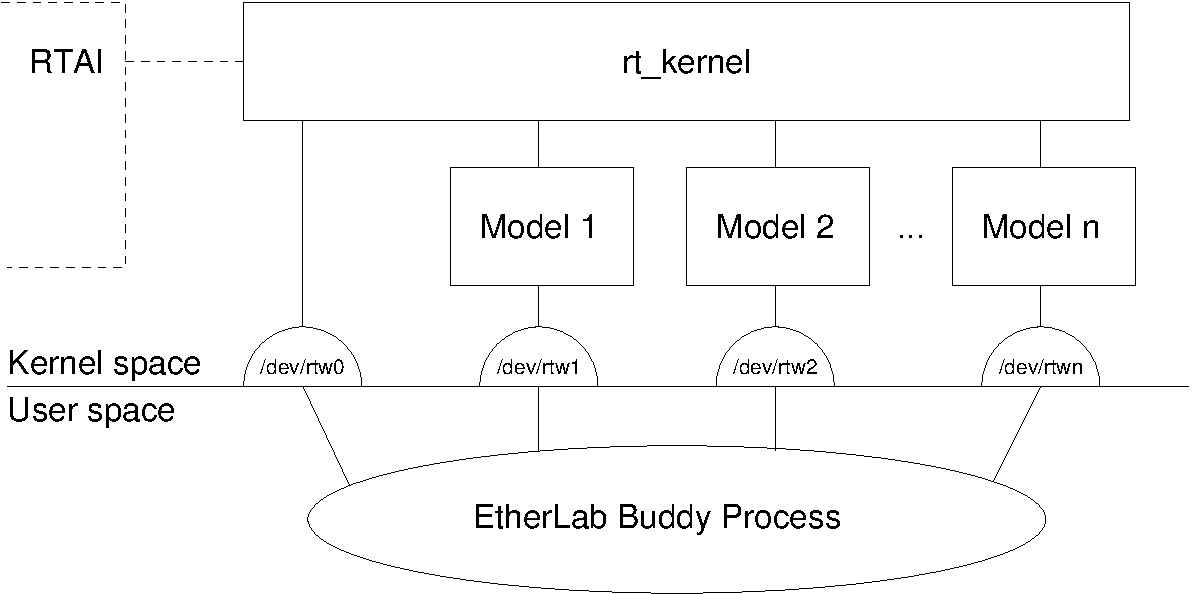
\includegraphics[width=\textwidth]{images/etl-arch}
    \caption{EtherLab runtime architecture}
    \label{fig:architektur}
  \end{center}
\end{figure}

\end{ighsec}

%-----------------------------------------------------------------------------

\begin{ighsec}{Installation}
\label{sec:install}

\begin{ighsec}{Prerequisites}

Prerequisites for the installation of EtherLab:

\begin{itemize}

\item Linux kernel 2.6 (including kernel sources)

\item RTAI $\ge$ 3.3

\item {\it optional:} MATLAB/Simulink with Realtime Workshop, if Simulink
shall be used to create EtherLab realtime applications. Recommended are MATLAB
versions 2006{\it x} -- 2007{\it x}.

\item {\it optional:} EtherCAT master 1.4, if the Simulink EtherCAT blocks
shall be used. See \url{http://etherlab.org/en/ethercat}.

\end{itemize}

It is recommended to install EtherLab components to \texttt{/opt/etherlab}. If
this directory does not exist, it can be created with the commands below:

\begin{lstlisting}[gobble=2]
  # `\textbf{mkdir /opt/etherlab}`
  # `\textbf{chown root:users /opt/etherlab}`
  # `\textbf{chmod 775 /opt/etherlab}`
\end{lstlisting}

\end{ighsec}

\begin{ighsec}{Installation}
\label{sec:inst-paket}

Installation is done after copying the EtherLab tarball from the EtherLab CD
(or downloading from \url{http://etherlab.org}) as normal user according to
the commands below. The last command installs EtherLab into the directory
\texttt{/opt/etherlab}. A different target directory can be selected via the
\texttt{--prefix} parameter of the \texttt{configure} script (see
\texttt{configure --help}).

\begin{lstlisting}[gobble=2]
  `\$` `\textbf{tar xzf etherlab-\version.tar.gz}`
  `\$` `\textbf{cd etherlab-\version/}`
  `\$` `\textbf{./configure}`
  `\$` `\textbf{make}`
  `\$` `\textbf{make install}`
\end{lstlisting}

\end{ighsec}

\begin{ighsec}{Installation of the Simulink Library}
\label{sec:inst-blockset}

As a prerequisite for the \texttt{setup\_etherlab} command (see below) to
succeed, the file \texttt{toolbox/local/pathdef.m} inside the MATLAB
installation directory must be writable for the user running MATLAB. Enter the
below commands (as \textit{root}) to make it writable for all users in the
group \textit{users} (substitute the variable \texttt{\$MATLABDIR} with the
correct path first):

\begin{lstlisting}[gobble=2]
  # `\textbf{chown :users \$MATLABDIR/toolbox/local/pathdef.m}`
  # `\textbf{chmod 664 \$MATLABDIR/toolbox/local/pathdef.m}`
\end{lstlisting}

To setup the EtherLab Simulink library \texttt{etherlab\_lib} for the use in
MATLAB, the below commands must be entered (out of MATLAB).

\begin{lstlisting}[gobble=2]
  >> `\textbf{cd /opt/etherlab/rtw}`
  >> `\textbf{setup\_etherlab}`
\end{lstlisting}

\end{ighsec}

\begin{ighsec}{Starting EtherLab as a Service}
\label{sec:dienst}

If the EtherLab kernel/buddy are to be started as a service, the provided init
script \texttt{etherlab} can be used. However, the insertion of the service is
dependent on the GNU/Linux distribution used. The command sequence below is
intended for openSUSE Linux:

\begin{lstlisting}[gobble=2]
  # `\textbf{ln -s /opt/etherlab/etc/init.d/etherlab /etc/init.d/}`
  # `\textbf{insserv etherlab}`
\end{lstlisting}

\end{ighsec}

\end{ighsec}

%-----------------------------------------------------------------------------

\begin{ighsec}{The EtherLab C-API}
\label{sec:api}

\begin{ighsec}{Concept}
\label{sec:api-concept}

EtherLab provides a generic way of executing realtime applications in the
Linux kernel and accessing their signals and parameters from userspace. The
EtherLab C-API provides functions to

\begin{itemize}

\item Initialize and clean up realtime applications.

\item Accept information about the internal structure of a realtime
application, i.\,e.\,application attributes, different tasks, signals and
parameters, to allow access from userspace.

\item Execute an application's tasks with different sample times.

\end{itemize}

The realtime application description is done via an XML file (see
section~\ref{sec:xml}). This file is parsed to create the C data structures
for signals and parameters. This means the user only has to provide the
application description XML and the C-code algorithms operating on the given
data structures to create an EtherLab realtime application. The
\texttt{rt\_kernel} provides machanisms to make the application's variables
visible and accessible in userspace. See section~\ref{sec:build} on how to
build a basic application.

\end{ighsec}

\begin{ighsec}{Realtime Application Description XML}
\label{sec:xml}

Listing~\ref{lst:min-desc} shows a minimal realtime application description.

\begin{lstlisting}[caption={Minimal realtime application description},
    label={lst:min-desc}]
<?xml version="1.0"?>
<application>
  <description>EtherLab example application</description>
  <version>Version string</version>
  <task basetick="1000"/>
  <data>
    <signal name="signal1" datatype="double_T"/>
    <parameter name="parameter1" datatype="double_T"/>
  </data>
</application>
\end{lstlisting}

\begin{ighsec}{The application element}
\label{sec:xml-app}

The root of the realtime application description XML is the
\texttt{<application>} element. It may contain the following elements (the
order is mandatory).

\begin{description}

\item[\small\texttt{<description>}] (\textit{mandatory}) May contain an
arbitrary textual description of the application. Please note, that this
results in a C string, so please avoid doublequotes and \lstinline+\0+.

\item[\small\texttt{<version>}] (\textit{mandatory}) May contain an arbitrary
version string. The same constraints as for the \texttt{<description>}
element apply.

\item[\small\texttt{<task>}] (\textit{mandatory}) This sets the base period of
the application's main task. The period is set via the \texttt{basetick}
attribute, that is interpreted as time period in \textmu s and will be later
referenced as sample time index 0. The element may optionally have
\texttt{<subtask>} child elements with a mandatory \texttt{decimation}
attribute. Each of them will create a subtask with an execution period of the
application's base period divided by the given decimation.

\item[\small\texttt{<refsystem>}] (\textit{optional}) Reference systems serve
as target systems for \texttt{<reference>} elements, that can appear in
system-like elements (see section~\ref{sec:xml-system}). The element itsself
is a system-like element. An arbitrary number of reference systems can be
defined in this place.

\item[\small\texttt{<data>}] (\textit{mandatory}) This is the root of the
application's data structure and can be considered as a system-like element
(see section~\ref{sec:xml-system}).

\end{description}

\end{ighsec}

\begin{ighsec}{System-like elements}
\label{sec:xml-system}

The elements \texttt{<data>}, \texttt{<subsystem>} and \texttt{<refsystem>}
can be considered as system-like elements, that behave similar in a certain
way.  Below is a list of elements that can appear as child elements in
system-like elements. System-like elements can contain subsystems in terms of
the \texttt{<subsystem>} or \texttt{<reference>} elements, so that nested tree
structures can be created. Each node is identified by a name. As a result, any
children of system-like elements must have a unique \texttt{name} attribute.

\begin{description}

\item[\small\texttt{<signal>}] Defines a signal as part of the parent system.
A signal is a variable, that is calculated at a given sample time. See
section~\ref{sec:vars} for more information on variables. The element can
accept the following attributes:

\begin{description}

\item[\small\texttt{name}] (\textit{mandatory}) The name of the signal. This
must be a valid C variable name.

\item[\small\texttt{datatype}] (\textit{mandatory}) One of the variable data
types listed in section~\ref{sec:vars}.

\item[\small\texttt{sampleTimeIndex}] (\textit{optional}) The index of the
sample time referencing the task or subtask defined in the application (see
section~\ref{sec:xml-app}). This also specifies the fastest rate of change for
the signal. If \texttt{sampleTimeIndex} is ommitted, the signal will belong to
the fastest sample time.

\item[\small\texttt{alias}] (\textit{optional}) An alternate global name for
the signal.

\end{description}

\item[\small\texttt{<parameter>}] Defines a parameter variable as part of the
parent system. As far as the application is concerned, a parameter is a
constant value. It is only possible to change the value via external
mechanisms provided by \texttt{rt\_kernel}. See section~\ref{sec:vars} for
more information on variables. The following attributes are possible for this
element:

\begin{description}

\item[\small\texttt{name}] (\textit{mandatory}) The name of the parameter.
This must be a valid C variable name.

\item[\small\texttt{datatype}] (\textit{mandatory}) One of the variable data
types listed in section~\ref{sec:vars}.

\end{description}

\item[\small\texttt{<subsystem>}] A subsystem will create a deeper nesting
level and a new namespace for signals, parameters and further subsystems. The
\texttt{name} attribute defines the name of the subsystem and is therefore
mandatory. A subsystem will result in an unnamed C structure. If a named data
structure is required, use \texttt{<reference>} instead.

\item[\small\texttt{<reference>}] A reference will create a subsystem as an
instance of a \texttt{<refsystem>} (see section~\ref{sec:xml-app}). The
\texttt{name} attribute defines the name of the subsystem and therefore is
mandatory. A reference will create a named C structure, that can be used as a
data type in C code (for example as a function parameter's type).

\end{description}

\end{ighsec}

\begin{ighsec}{Variables}
\label{sec:vars}

Signals and parameters are considered as variables. Variables are the
''leaves'' of the tree of systems defined in the application's \texttt{<data>}
section and are the elements that make up the realtime application's data.

The available variable data types are listed below:

\begin{center}
\begin{tabular}{|l|l|}
EtherLab name & Size in byte\\\hline\hline
\lstinline+uint8_T+ & 1\\
\lstinline+sint8_T+ & 1\\
\lstinline+int16_T+ & 2\\
\lstinline+sint16_T+ & 2\\
\lstinline+uint32_T+ & 4\\
\lstinline+sint32_T+ & 4\\
\lstinline+float_T+ & 4\\
\lstinline+double_T+ & 8\\\hline
\end{tabular}
\end{center}

Due to their special character, variables may be described with the below
child elements in the application description XML. The order is mandatory
again.

\begin{description}

\item[\small\texttt{<dim>}] (\textit{optional}) A variable can be
multi-dimensional. Any \texttt{<dim>} element will add another dimension to
the variable. If ommitted, the variable is considered as a scalar. Every
\texttt{<dim>} element has a mandatory \texttt{value} attribute, that
specifies the size of the dimension. For example

\begin{lstlisting}
<signal name="matrix" datatype="double_T">
  <dim value="5"/>
  <dim value="7"/>
</signal>
\end{lstlisting}

will create a signal named \texttt{matrix} that is a $5\times7$ matrix of
double-precision floating-point values, so the resulting C variable will be
defined as \lstinline{double_T matrix[5][7];}.

\item[\small\texttt{<value>}] (\textit{optional}) Default values may be
specified for variables on application startup. If the variable is a scalar, a
single element (for example \lstinline+<value>8</value>+) will be sufficient.
If the variable is multi-dimensional, the elements can be nested according to
the dimensions, like in the example below. If a \texttt{<value>} element is
ommitted, if will default to zero.

\begin{lstlisting}
<parameter name="matrixParam" datatype="uint8_T">
  <dim value="2"/>
  <dim value="3"/>
  <value>
    <value>
      <value>1</value>
      <value>2</value>
      <value>3</value>
    </value>
    <value>
      <value>4</value>
      <value>5</value>
      <value>6</value>
    </value>
  </value>
</signal>
\end{lstlisting}

\item[\small\texttt{<meta>}] (\textit{optional}) Variables can have additional
information attached. These are not precisely specified and can be arbitrary
strings. This has to be defined in the future.

\end{description}

\end{ighsec}

\end{ighsec}

\begin{ighsec}{Building a Model}
\label{sec:build}

\end{ighsec}

\end{ighsec}

%-----------------------------------------------------------------------------

\begin{ighsec}{Simulink Integration}
\label{sec:simulink}

%-----------------------------------------------------------------------------

\begin{ighsec}{The Simulink Library}
\label{sec:lib}

The EtherLab library \texttt{etherlab\_lib} was designed to allow the creation
of EtherLab applications using MATLAB/Simulink models. For example, it
contains Simulink blocks for all supported EtherCAT slaves. To show the
library window (see figure~\ref{fig:blockset}), the command below have to be
entered in MATLAB:

\begin{lstlisting}[gobble=2]
  >> `\textbf{etherlab\_lib}`
\end{lstlisting}

Figure~\ref{fig:blockset} shows the window containing the
\texttt{etherlab\_lib} with the EtherCAT blockset. Each block has a
configuration dialog, that shows up after double-clicking on the block area.
There is a ``Help'' button in all of the configuration dialogs, that provides
detailed help concerning the dialog elements.

\begin{figure}[H]
  \begin{center}
    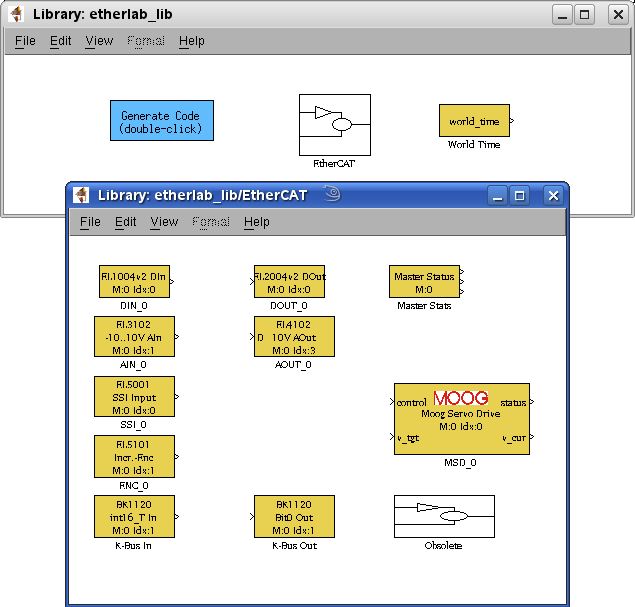
\includegraphics[width=0.9\textwidth]{images/blockset.png}
    \caption{EtherLab Simulink Blockset}
    \label{fig:blockset}
  \end{center}
\end{figure}

Figure~\ref{fig:el10xx} shows the configuration dialog for the
digital-input EtherCAT slaves of the Beckhoff EL10XX series.

\begin{figure}[H]
  \begin{center}
    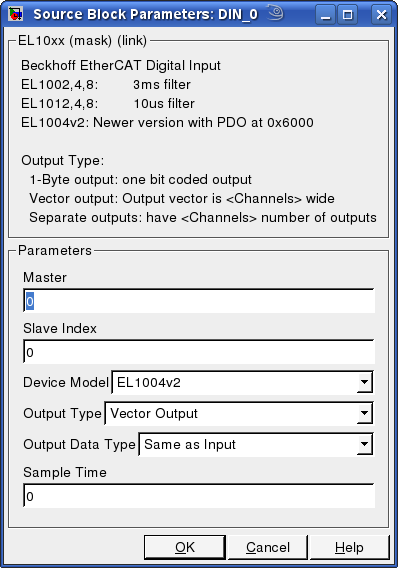
\includegraphics[width=0.4\textwidth]{images/el10xx.png}
    \caption{EL10xx configuration dialog}
    \label{fig:el10xx}
  \end{center}
\end{figure}

Figure~\ref{fig:el20xx} shows the configuration dialog for the
digital-output EtherCAT slaves of the Beckhoff EL20XX series.

\begin{figure}[H]
  \begin{center}
    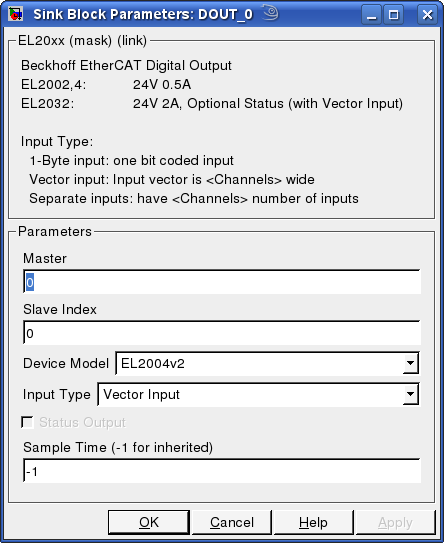
\includegraphics[width=0.4\textwidth]{images/el20xx.png}
    \caption{EL20xx configuration dialog}
    \label{fig:el20xx}
  \end{center}
\end{figure}

Figure~\ref{fig:el31xx} shows the configuration dialog for the
analog-input EtherCAT slaves of the Beckhoff EL31XX series.

\begin{figure}[H]
  \begin{center}
    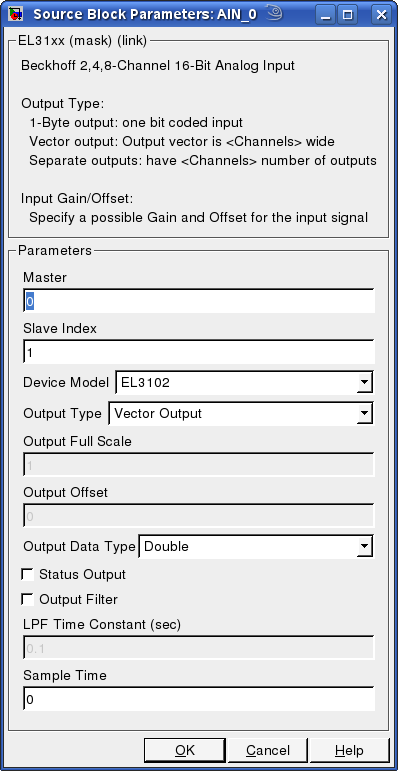
\includegraphics[width=0.4\textwidth]{images/el31xx.png}
    \caption{EL31xx configuration dialog}
    \label{fig:el31xx}
  \end{center}
\end{figure}

Figure~\ref{fig:el41xx} shows the configuration dialog for the
analog-output EtherCAT slaves of the Beckhoff EL41XX series.

\begin{figure}[H]
  \begin{center}
    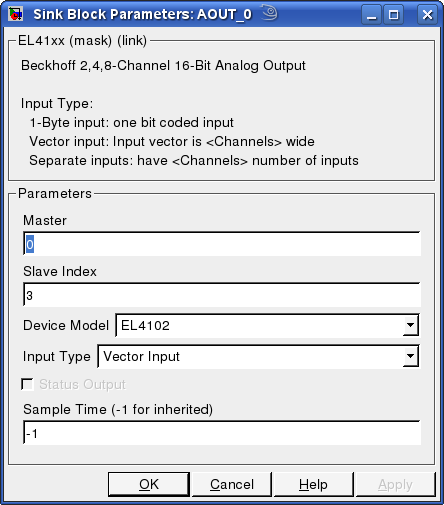
\includegraphics[width=0.4\textwidth]{images/el41xx.png}
    \caption{EL41xx configuration dialog}
    \label{fig:el41xx}
  \end{center}
\end{figure}

Figure~\ref{fig:el5001} shows the configuration dialog for the SSI
EtherCAT slave Beckhoff EL5001.

\begin{figure}[H]
  \begin{center}
    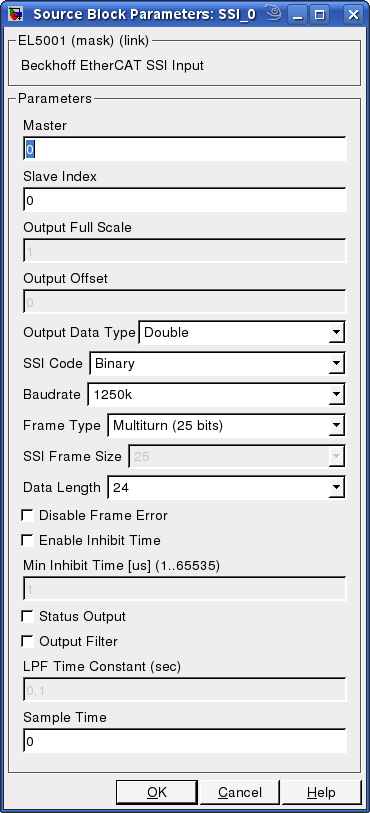
\includegraphics[width=0.4\textwidth]{images/el5001.png}
    \caption{EL5001 configuration dialog}
    \label{fig:el5001}
  \end{center}
\end{figure}

Figure~\ref{fig:el5101} shows the configuration dialog for the
incremental-encoder EtherCAT slave Beckhoff EL5101.

\begin{figure}[H]
  \begin{center}
    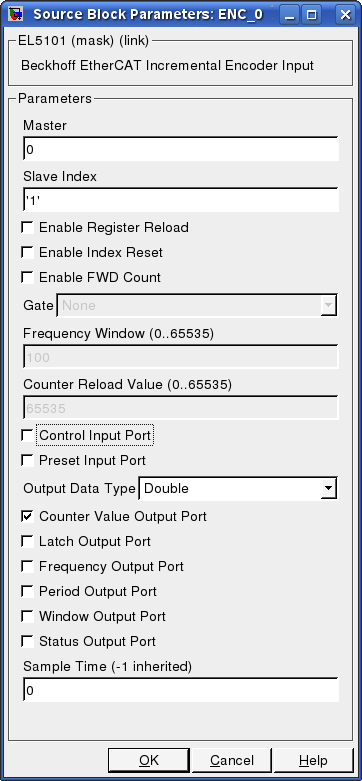
\includegraphics[width=0.4\textwidth]{images/el5101.png}
    \caption{EL5101 configuration dialog}
    \label{fig:el5101}
  \end{center}
\end{figure}

Figure~\ref{fig:bk1120-in} shows the configuration dialog for the Beckhoff
BK1120 EtherCAT-KBUS-coupler input block.

\begin{figure}[H]
  \begin{center}
    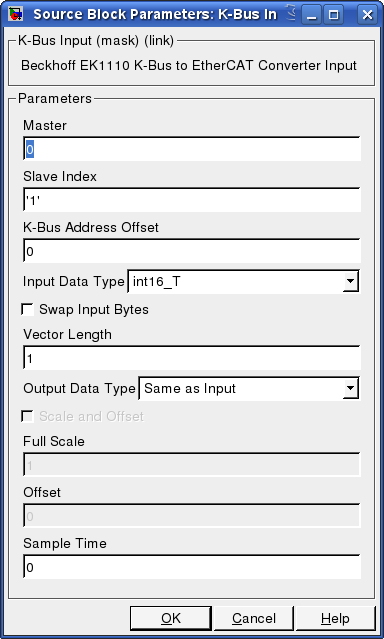
\includegraphics[width=0.4\textwidth]{images/bk1120-in.png}
    \caption{BK1120 input configuration}
    \label{fig:bk1120-in}
  \end{center}
\end{figure}

Figure~\ref{fig:bk1120-out} shows the configuration dialog for the Beckhoff
BK1120 EtherCAT-KBUS-coupler output block.

\begin{figure}[H]
  \begin{center}
    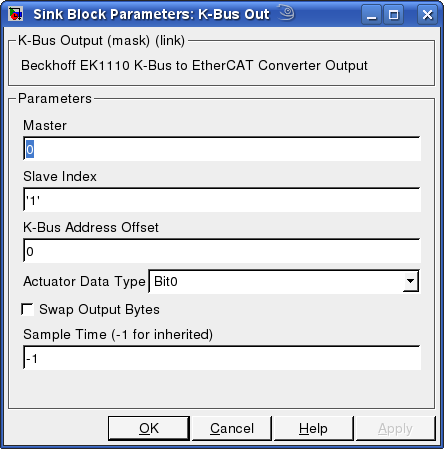
\includegraphics[width=0.4\textwidth]{images/bk1120-out.png}
    \caption{BK1120 output configuration}
    \label{fig:bk1120-out}
  \end{center}
\end{figure}

Figure~\ref{fig:msd} shows the configuration dialog for the MOOG servo drive
EtherCAT slave block. This block can be configured to be an input-only block,
an output-only block or and input/output block.

\begin{figure}[H]
  \begin{center}
    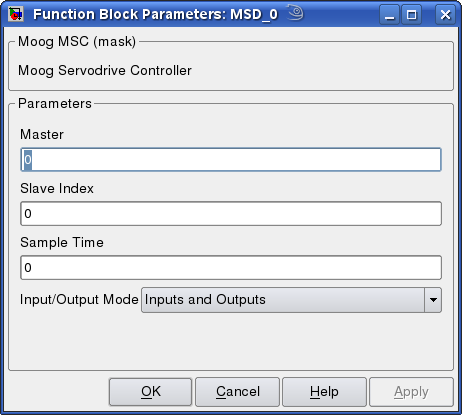
\includegraphics[width=0.4\textwidth]{images/moog_msd.png}
    \caption{MOOG servo drive configuration}
    \label{fig:msd}
  \end{center}
\end{figure}

Figure~\ref{fig:masterstats} shows the configuration dialog for the EtherCAT
master status block.

\begin{figure}[H]
  \begin{center}
    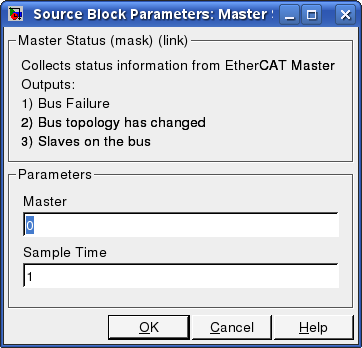
\includegraphics[width=0.4\textwidth]{images/master.png}
    \caption{Master status block configuration}
    \label{fig:masterstats}
  \end{center}
\end{figure}

\end{ighsec}

%-----------------------------------------------------------------------------

\begin{ighsec}{Creation of EtherLab Applications with Simulink}
\label{sec:simu-apps}

After creating a new model sheet within Simulink, a few parameters have to be
set up (menu \textit{Simulation/Configuration Parameters\ldots}):

\begin{itemize}
\item The input field \textit{Realtime Workshop} $\rightarrow$
  \textit{System target file} must contain the file name
  \texttt{etherlab.tlc}. It can be chosen via the
  \textit{Browse\ldots} button (see figure~\ref{fig:konfiguration}).
  \begin{figure}[H]
    \begin{center}
      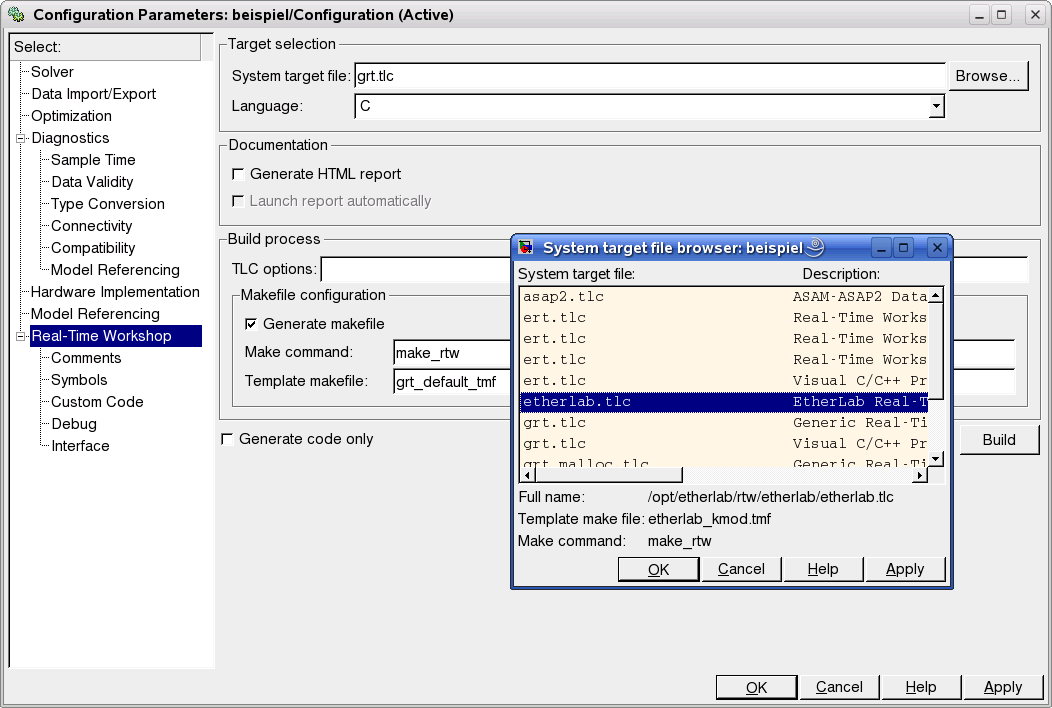
\includegraphics[width=.9\textwidth]{images/config_param.png}
      \caption{Configuration of model parameters}
      \label{fig:konfiguration}
    \end{center}
  \end{figure}
\item The input field \textit{Solver} $\rightarrow$ \textit{Fixed-step
    size} must contain the period time of the real time cycle, for
  example \texttt{0.01} meaning $100$ Hz (see
  figure~\ref{fig:config_solver}).
  \begin{figure}[H]
    \begin{center}
      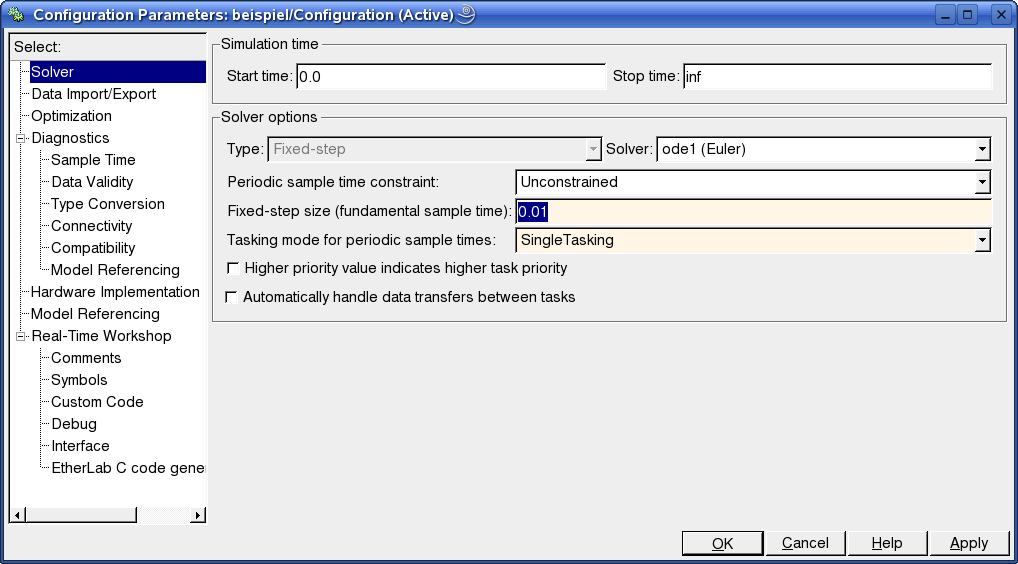
\includegraphics[width=.9\textwidth]{images/config_solver.png}
      \caption{Configuration of model parameters (2)}
      \label{fig:config_solver}
    \end{center}
  \end{figure}
\end{itemize}

After the model has been parametrized, it can be edited as usual. To use
EtherLab blocks, open the \texttt{etherlab\_lib} (see sec.~\ref{sec:lib}) and
drag the desired blocks on the new model sheet. When finished, \textit{Ctrl-B}
will generate the application code contained a Linux kernel module.

\end{ighsec}

%-----------------------------------------------------------------------------

\end{ighsec} % Simulink

%-----------------------------------------------------------------------------

\begin{ighsec}{Starting EtherLab Models}
\label{sec:start}

The \texttt{rt\_kernel} module must be inserted before inserting any EtherLab
modules. If EtherLab is configured as a service (see
section~\ref{sec:dienst}), this is done automatically at system startup.
Otherwise the module can be inserted manually. It is recommended to start the
module using the init script, because the necessary device files are then
created automatically:

\begin{lstlisting}[gobble=2]
  # `\textbf{/opt/etherlab/etc/init.d/etherlab start}`
\end{lstlisting}

After that, an EtherLab module can be loaded.

\begin{lstlisting}[gobble=2]
  # `\textbf{insmod <application>\_kmod.ko}`
\end{lstlisting}

If the \texttt{insmod} command returns with an error, the kernel ring
buffer can be analyzed for possible software or hardware
misconfigurations:

\begin{lstlisting}[gobble=2]
  # `\textbf{dmesg | less}`
\end{lstlisting}

If the application was loaded successfully, its variables (i.\,e.\,signals
and parameters) can ve accessed via TCP/IP with EtherLab tools like
Testmanager, DLS or the RTCom library (have a look at
\url{http://etherlab.org/en/components.php}. Therefore the
\texttt{etherlab\_buddy} acts as a TCP server listening on port 2345 and
communicating with an XML-based protocol called MSR (see the german
documentation at \url{http://etherlab.org/download/m-igh_rt_api.pdf}).

\end{ighsec}

%-----------------------------------------------------------------------------
